
\begin{enumerate}
\item 
\question{In Figure~\ref{figMultipleSwitches}, calculate the amount of current used by the whole circuit for each configuration of the switches S2 and S3 when S1 is closed.  You can assume that the LEDs are red LEDs.}
\solution{\begin{description}
\item[S2 closed] 9\mymamp 
\item[S3 closed] 4.5\mymamp
\item[Both closed] 13.5\mymamp
\end{description}}
\explanation{Because these circuit branches are in parallel, the total current is the sum of the individual currents.  
Because both branches connect to both positive and negative without going through resistance, then they each start at $9\myvolt$ and connect to ground, so they each use a full $9\myvolt$.
Therefore, we can use Ohm's Law to calculate the amount of current going through each branch:
\begin{align*}
I_{S2} &= V / R \\
       &= 9 / 1000 \\
       &= 0.009\myamp = 9\mymamp \\
I_{S3} &= V / R \\
       &= 9 / 2000 \\
       &= 0.0045\myamp = 4.5 \mymamp
\end{align*}
Therefore, when S2 is closed, that branch uses $9\mymamp$ of current, and when S3 is closed that branch uses $4.5\mymamp$ of current.
Since they are in parallel and both connected on both sides to the battery, when they are closed they both use $9 + 4.5 = 13.5\mymamp$ of current.
}
\item 
\question{Build the circuit given in Figure~\ref{figMultipleSwitches} (you may swap out resistors with different but similar values---anything from $300\myohm$ to about $5\mykohm$ should work).}
\solution{Since this is a building exercise, the question is whether or not it works correctly.}
\item 
\question{Given a $15\myvolt$ voltage supply, what size of a resistor would be needed to make sure that a circuit never went over $18\mymamp$.}
\solution{$833.33\myohm$}
\explanation{This can be figured out using Ohm's Law.  We simply figure out the resistance needed for $18\mymamp$ ($0.018\myamp$).
\begin{align*}
R &= V / I \\
  &= 15 / 0.018 \\
  &= 833.33\myohm
\end{align*}
}
\item 
\question{Given a $9\myvolt$ battery source, design a voltage divider that will output $7\myvolt$ to a load that has a resistance of $10\mykohm$.}
\solution{The general voltage divider circuit can be seen here:
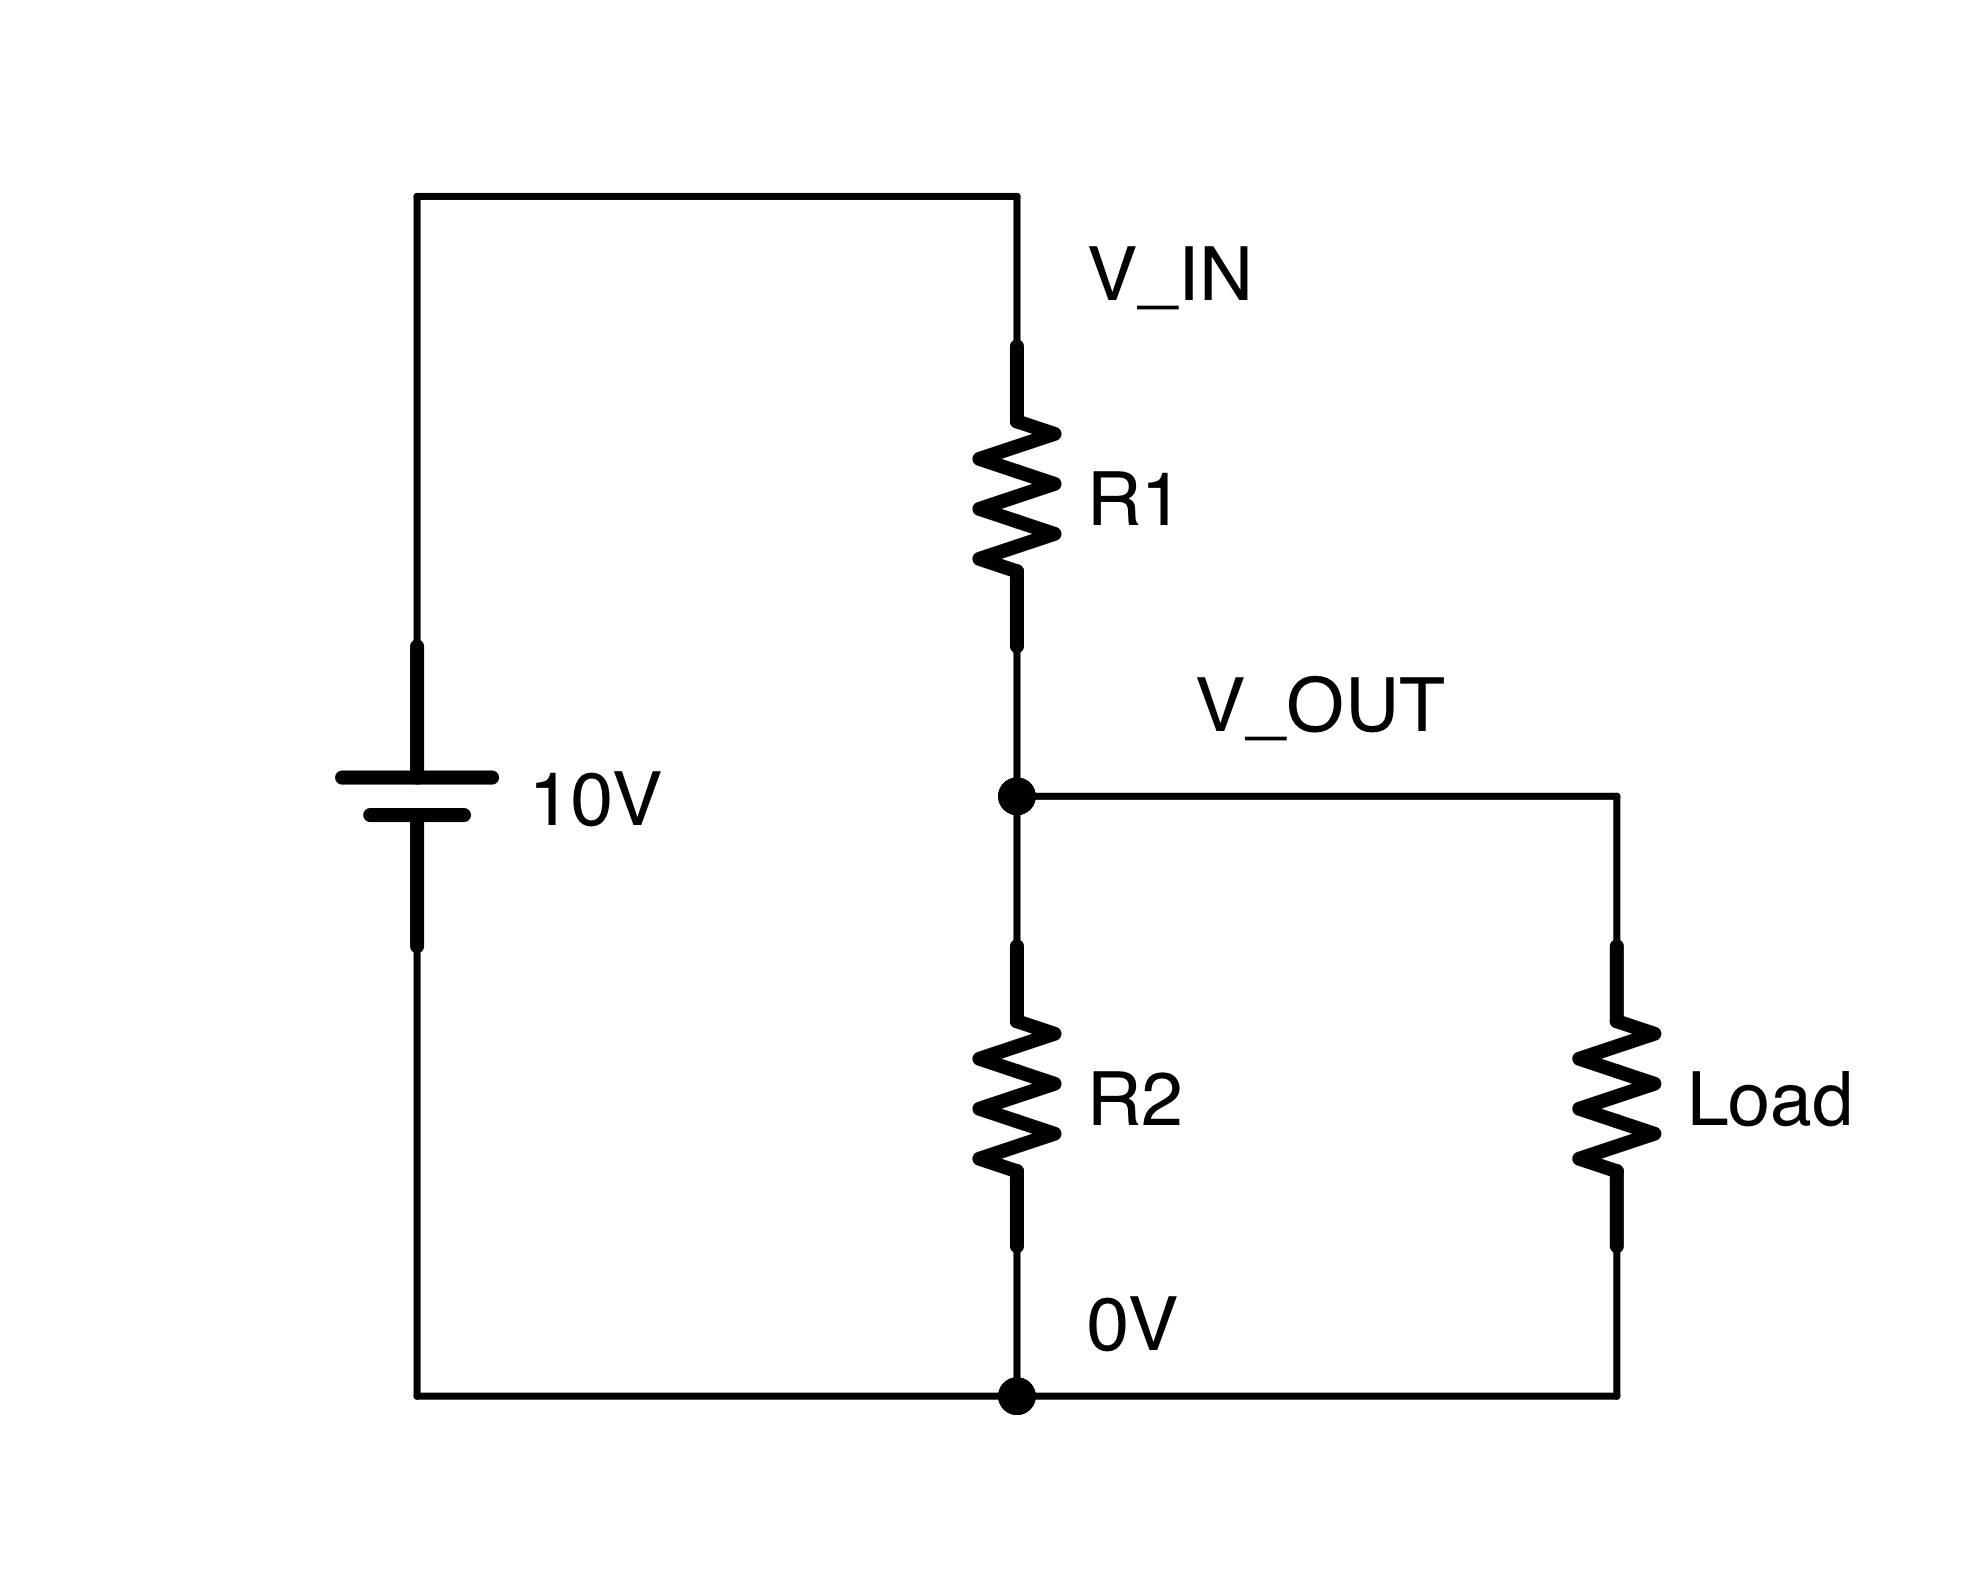
\includegraphics[width=\columnwidth]{ExVoltageDivider.png}
To achieve the required design, we need $R_1$ to be $428.57\myohm$ and $R_2$ to be $1,000\myohm$.}
\explanation{To create a voltage divider, we have to divide voltages between two resistors, with the output going out from between them.
Equation~\ref{eqVoltageDivision} shows us what the calculation looks like:
$$ V_{OUT} = V_{IN} * \frac{R_2}{R_1 + R_2} $$
Now, this equation only tells us about the ratio of the resistors, not what their specific value is.
For an equation for specific values for the resistors, we need to look at Equations~\ref{eqVDIVR2Eq} and~\ref{eqVDIVR1Eq}.
Equation~\ref{eqVDIVR2Eq} says:
\begin{align*}
R_2 &= R_L / 10 \\
    &= 10,000 / 10 \\
    &= 1,000\myohm
\end{align*}
Equation~\ref{eqVDIVR1Eq} says:
\begin{align*}
R_1 &= \frac{R_2 * (V_{IN} - V_{OUT})}{V_{OUT}} \\
    &= \frac{1,000 * (10 - 7)}{10} \\
    &= \frac{3,000}{7} \\
    &= 428.57\myohm
\end{align*}
Therefore, $R_1$ needs to be about $428.57\myohm$ and $R_2$ needs to be about $1,000\myohm$.
In reality, we would probably find a resistor that is close to $429\myohm$ even if it isn't exact.
Even a $400\myohm$ resistor would give a voltage within a few percent of the desired value.
}
\item 
\question{Given a $3\myvolt$ battery source, design a voltage divider that will output $1.5\myvolt$ to a load that has a resistance of $1\mykohm$.}
\solution{For this voltage divider, both $R_1$ and $R_2$ will be $100\myohm$.}
\explanation{Using the same equations as before, we can easily design a voltage divider. $R_2$ is determined by:
\begin{align*}
R_2 &= R_L / 10 \\
    &= 1,000 / 10 \\
    &= 100\myohm
\end{align*}
$R_1$ is determined by:
\begin{align*}
R_1 &= \frac{R_2 * (V_{IN} - V_{OUT})}{V_{OUT}} \\
    &= \frac{100 * (3 - 1.5)}{1.5} \\
    &= \frac{150}{1.5} \\
    &= 100\myohm
\end{align*}
Therefore, both $R_1$ and $R_2$ will be $100\myohm$.
}
\item 
\question{In Figure~\ref{figPullUpResistorBasic}, how much current is going through the circuit when the switch is open?  How much when it is closed?  You can assume that the LED is a red LED.}
\solution{The circuit uses $7.2\mymamp$ of current when the switch is open and $9\mymamp$ when the switch is closed.}
\explanation{When the switch is open, the current passes through \emph{both} the resistor and the LED.
Therefore, we have to account for the voltage drop of the LED itself as well as the resistance.
The starting voltage is $9\myvolt$ and a red LED will give a voltage drop of $1.8\myvolt$.
Therefore, the remaining voltage through the resistor will be $9 - 1.8 = 7.2\myvolt$.
Using Ohm's Law, we can find out the current flow:
\begin{align*}
I &= V / R \\
  &= 7.2 / 1,000 \\
  &= 0.0072\myamp = 7.2\mymamp
\end{align*}
Therefore, when the switch is open, the circuit consumes $7.2\mymamp$.
When it is closed, the current does \emph{not} flow through the LED.
The reason is that since there is a direct connection between the resistor and the ground, then the resistor \emph{must} be at a zero-volt state at the end of it.
Therefore, there is no voltage remaining to push through the LED.

Therefore, the entire $9\myvolt$ is flowing across the resistor.
This means that the calculation for Ohm's Law is as follows:
\begin{align*}
I &= V / R \\
  &= 9 / 1,000 \\
  &= 0.009 \myamp = 9\mymamp
\end{align*}
Therefore, when the switch is closed, the circuit uses $9\mymamp$ of current.
}
\item 
\question{How would you modify the circuit in Figure~\ref{figPullUpResistorBasic} to keep the maximum current in the circuit under $2\mymamp$?  Draw the full circuit out yourself.}
\solution{The full circuit should look like the below drawing:
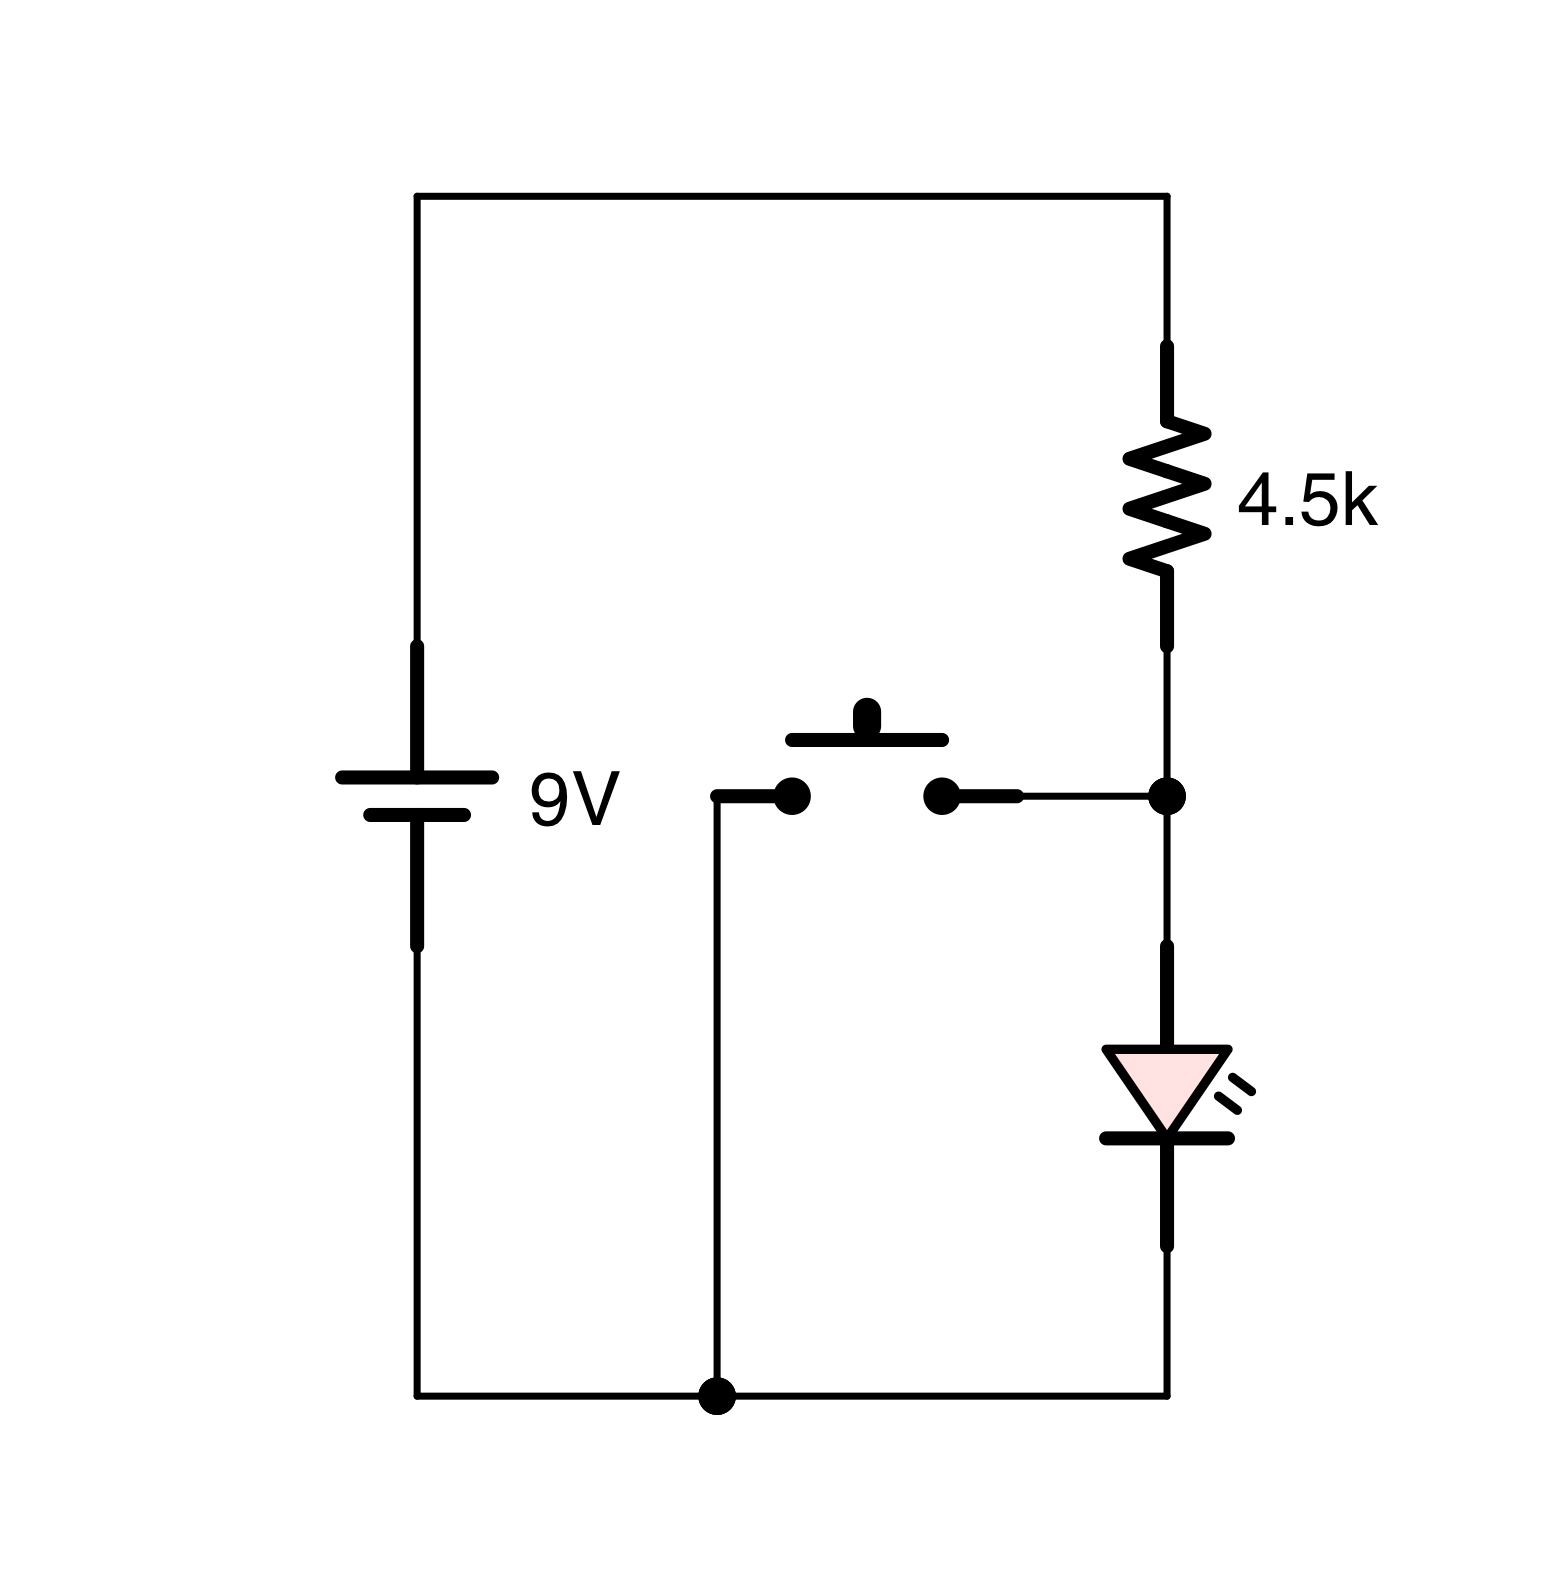
\includegraphics[width=\columnwidth]{ExPullUpResistorBasic.png}
}
\explanation{As we saw in the previous question, the circuit actually uses \emph{more} current when the switch is closed than when it is open.
Therefore, if we want to max sure the current never goes over $2\mymamp$ ($0.002\mymamp$), then we should design for that when the circuit is closed.
Therefore, using Ohm's Law, we can solve for the needed resistance like this:
\begin{align*}
R &= V / I \\
  &= 9 / 0.002 \\
  &= 4,500\myohm
\end{align*}
The drawn circuit should be identical to Figure~\ref{figPullUpResistorBasic} but with a $4,500\myohm$ resistor.
}
\item 
\question{Build the circuit you designed in the previous question.  If you do not have the right resistor values, use the closest ones you have.}
\solution{This is a project-building exercise.  The solution is correct if pushing the button turns off the light.  The one potential problem is if pushing the button creates a short circuit.  If this happens the project will get hot quickly.}
\end{enumerate}
